\documentclass[../main.tex]{subfiles}

\begin{document}

\section{Problem 1}

A square disc with sides \SI{7}{\milli\meter} is made out of a piezoelectric material having a strain coefficient of \SI{550d-12}{\meter\per\volt} and a mechanical compliance of \SI{20d-12}{\meter\squared\per\newton}. 
Compute (a) the strain produced by a force of \SI{50}{\newton} applied to the face of the material when the applied electric field is zero, and (b) the electric field required to produce an equivalent amount of strain when the applied stress is equal to zero.


\paragraph{a)} To compute the strain produce by a given force we can use the mechanical compliance and the following relation,
\begin{gather*}
    S = \frac{1}{\xi}T,
\end{gather*}
where $S$ is the elongation, $T$ the applied force and $1/\xi$ is the mechanical compliance.
Hence, replacing with numeric values,
\begin{align*}
    S &= \SI[per-mode=fraction]{20d-12}{\meter\squared\per\newton}\SI{50}{\newton} \\
      &= \SI{1d-9}{\meter\squared}.
\end{align*}

Since the strain is a dimensionless quantity, we need to take the ratio between the deform area and the origina area,
\begin{align*}
    S &= \frac{\SI{1d-9}{\meter\squared}}{\SI{49d-6}{\meter\squared}} \\
      &= \frac{1}{49}\times\num{d-3}. 
\end{align*}

\paragraph{b)}\label{par:1.b} Finally, in order to compute the required electric field to produce a previous strain when the applied stress is zero, we can use the following coupling relation,
\begin{align*}
    S = \frac{1}{\xi}T + g E,
\end{align*}
where $S$ is the strain, $1/\xi$ is the mechanical compliance, $T$ is the stress, $g$ is the strain coefficient and $E$ the electric field.
Since the applied stress is zero, the relation simplifies to,
\begin{align*}
    S = g E.
\end{align*}
Solving for the electric field and replacing by the numeric values we get,
\begin{align*}
    E &= \frac{S}{g} \\
      &= \frac{\SI{550d12}{\volt\per\meter}}{\num{49d3}} \\
      &= \frac{550}{49}\times\SI[per-mode=fraction]{d9}{\volt\per\meter} \\
      &\approx \SI[per-mode=fraction]{11.224d9}{\volt\per\meter}, 
\end{align*}


\section{Problem 2}

Find out the dielectric permittivity of the above-mentioned sample if the piezoelectric coupling coefficient of the material is k = \num{0.7}.

\paragraph{Finding $\epsilon$} In order to compute the dielectric permittivity we use the following relation between the piezoelectric coupling coefficient ($k$), piezoelectric constant ($d$) and mechanical compliance ($1/\xi$),
\begin{align*}
    k^2 &= \frac{d^2}{1/\xi\epsilon} \\
\epsilon &= \frac{d^2}{1/\xi k^2}
\end{align*}
replacing the numeric values,
\begin{align*}
    \epsilon &= \frac{\left(\SI{550d-12}{\meter\per\volt}\right)^2}{\SI{20d-12}{\meter\squared\per\newton} (0.7)^2} \\
             &\approx \SI{3.086d-8}{\newton\per\volt\squared},
\end{align*}
Recalling that \SI{}{\volt} $=$ \SI{}{\newton\meter\per\coulomb}, we get,
\begin{gather*}
    \epsilon\approx \SI[per-mode=fraction]{3.086d-8}{\coulomb\squared\per\newton\per\meter\squared}
\end{gather*}

\section{Problem 3}

Compute the stress required to produce 100 microstrain in APC 856 when the applied electric field is held constant at zero. 
Assume that the material APC 856 has a compliance at constant electric field $s^E=\SI{15.3d-12}{\meter\squared\per\newton}$

\paragraph{Finding strain} This case is similar to problem\ref{par:1.b}.
Hence, we can applied the same constitutive equation for small deformations and compute the stress,
\begin{align*}
    S &= \frac{1}{\xi}T + \cancelto{0}{g E} \\
    T &= \xi S \\
      &= \frac{1}{\SI{15.3d-12}{\meter\squared\per\newton}}\num{100d-6} \\
      &= \SI[per-mode=fraction]{6.535d6}{\newton\per\meter\squared}
\end{align*}


\section{Problem 4}

(a) What do you understand by centrosymmetric crystal? 
(b) Explain with suitable diagram/s why piezoelectricity is not observed in all types of crystals while electrostriction is observed in all crystals.

\paragraph{Centrosymmetric crystals} The representation of a crystal material as a lattice allows to understand the ``centrosymmetric'' as a symmetry in the lattice.
This is an inversion center type of symmetry.
Therefore, if each point's coordinates are inverted, $(x,y,z)\to(-x,-y,-z)$, the point remains unchanged.

\paragraph{Connection with electrostriction and piezoelectricity} 
On the other hand, electrostriction is an effect observe when an electric field is applied to a crystal and induces a deformation (strain) in the material.
When the crystal is represented by a centrosymmetric lattice and introduce a uniform deformation, the inversion symmetry cause that each atom position has an identical partern (fig~\ref{fig:2a}).
However, a piezoelectric material is represented by a lattice lacking of centrosymmetry.
This absecense of symmetry cause the creation of a dipole that can be measure as a voltage (fig~\ref{fig:2b}).
Although in figure~\ref{fig:centro} it is shown a hexagonal lattice, the detail of adding different type of particles it is crutial to break the symmetry.

\newpage

\begin{figure}[ht!]
    \centering
    \begin{subfigure}[c]{0.45\textwidth}
        \centering
        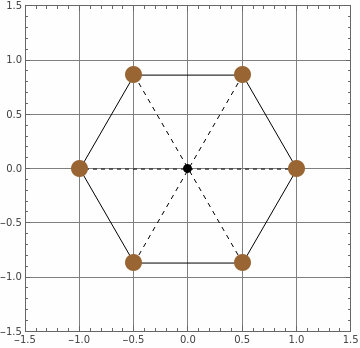
\includegraphics[width=\textwidth]{../imgs/img1a.png}
        \caption{~}\label{fig:1a}
    \end{subfigure}
    \begin{subfigure}[c]{0.45\textwidth}
        \centering
        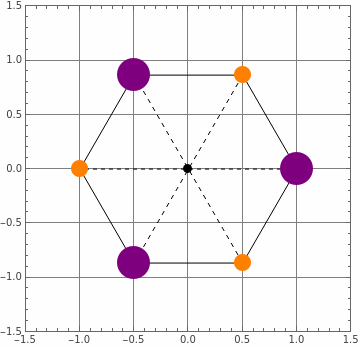
\includegraphics[width=\textwidth]{../imgs/img1b.png}
        \caption{~}\label{fig:1b}
    \end{subfigure}

    \begin{subfigure}[c]{0.45\textwidth}
        \centering
        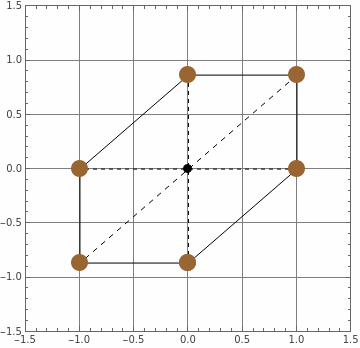
\includegraphics[width=\textwidth]{../imgs/img2a.png}
        \caption{~}\label{fig:2a}
    \end{subfigure}
    \begin{subfigure}[c]{0.45\textwidth}
        \centering
        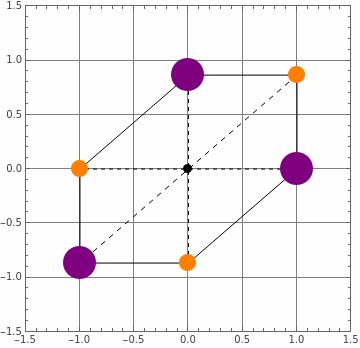
\includegraphics[width=\textwidth]{../imgs/img2b.png}
        \caption{~}\label{fig:2b}
    \end{subfigure}

    \caption{Representation of centrosymmetry lattice under deformation. Figures\ref{fig:1a} and~\ref{fig:2a} represent electrostriction is a non-piezoelectric material and figures\ref{fig:1b} and~\ref{fig:2b} represent electrostriction is a piezoelectric material}\label{fig:centro}
\end{figure}


\newpage

\section{Problem 5}

Do a survey and find out 5 companies that sell piezoelectric ceramics and piezoelectric polymers. 
List the specifications including the piezoelectric constants and unit price of these materials. 
You will need these materials for your final project so also find out which company will deliver the products here and what is the lead time.

\begin{figure}[ht!]
    \centering
    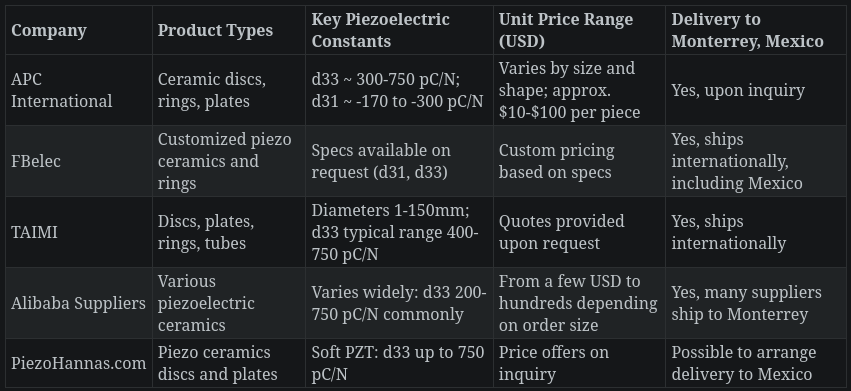
\includegraphics[width=0.9\textwidth]{../imgs/table.png}
\end{figure}

\end{document}
